\documentclass{article}
\usepackage[utf8]{inputenc}
\usepackage[spanish]{babel}
\usepackage{listings}
\usepackage{graphicx}
\usepackage{listings}
\usepackage{xcolor}
\graphicspath{ {images/} }
\usepackage{cite}
\definecolor{codegreen}{rgb}{0,0.6,0}
\definecolor{codegray}{rgb}{0.5,0.5,0.5}
\definecolor{codepurple}{rgb}{0.58,0,0.82}
\definecolor{backcolour}{rgb}{0.95,0.95,0.92}

\lstdefinestyle{mystyle}{
    backgroundcolor=\color{backcolour},   
    commentstyle=\color{codegreen},
    keywordstyle=\color{magenta},
    numberstyle=\tiny\color{codegray},
    stringstyle=\color{codepurple},
    basicstyle=\ttfamily\footnotesize,
    breakatwhitespace=false,         
    breaklines=true,                 
    captionpos=b,                    
    keepspaces=true,                 
    numbers=left,                    
    numbersep=5pt,                  
    showspaces=false,                
    showstringspaces=false,
    showtabs=false,                  
    tabsize=2
}
\lstset{style=mystyle}

\begin{document}

\begin{titlepage}
    \begin{center}
        \vspace*{1cm}
            
        \Huge
        \textbf{Informe implementación}
            
        \vspace{0.5cm}
        \LARGE
        Parcial 2
            
        \vspace{1.5cm}
        \textbf{Miguel Angel Serna Montoya\\CC 1193129865}
        
            
        \vfill
            
        \vspace{0.8cm}
            
        \Large
        Departamento de Ingeniería Electrónica y Telecomunicaciones\\
        Universidad de Antioquia\\
        Medellín\\
        Septiembre de 2021
            
    \end{center}
\end{titlepage}

\tableofcontents

\section{Clases implementadas} \label{contenido}
\subsection{lecturaEscritura}
Esta clase es la que se encarga de leer la imagen y almacenarla como un atributo privado. Una vez la imagen
es escalada esta recibe un vector 3d mediante un método publico y lo escribe en un txt que el usuario debe copiar.
\subsection{escalado}
Esta clase tiene como parámetro el ancho y alto de la imagen almacenada por lectura escritura. Mediante un método publico le entrego la imagen de lectura y esta trabajara para escalar la imagen a un tamaño de 8x8 mediante el método publico escalameEsta().
\subsection{Menuapp}
esta clase se encarga de crear las interacciones entre las 2 anteriores clases ya mencionadas. Posee un atributo privado de clase lecturaEscritura y otro atributo privado de escalado. Los inicializa en memoria dinámica en su constructor y allí trabaja con estos mismos.
\newpage
\section{Esquema de clases}
\begin{figure}[h]
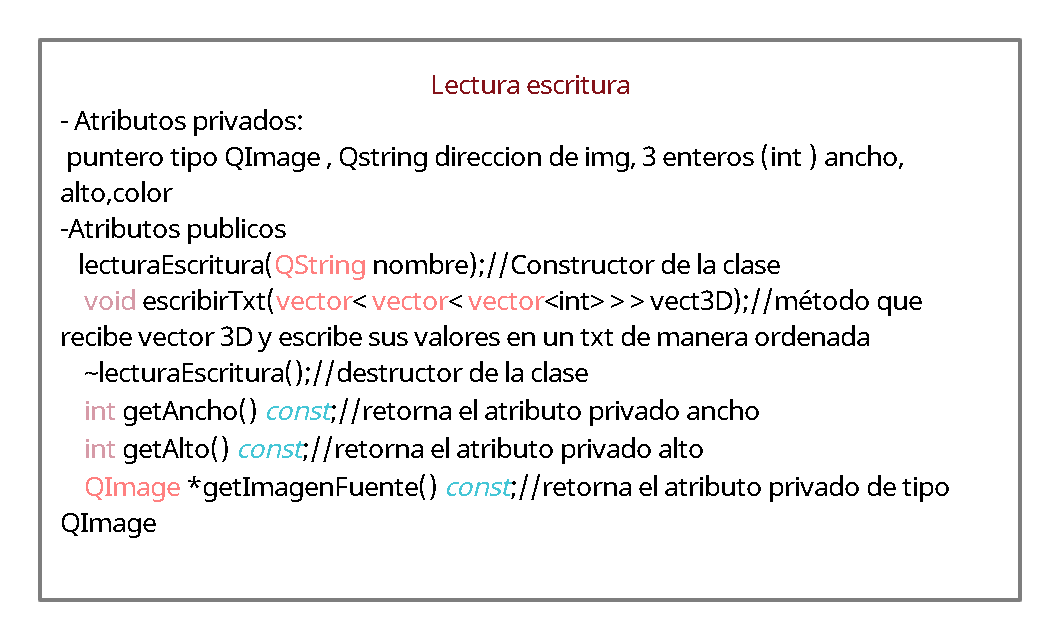
\includegraphics[width=8cm]{resources/esquemaLecturaEscritura.png}
\centering

\caption{esquema Clase lecturaEscritura}
\label{fig:RAMM}
\end{figure}
\begin{figure}[h]
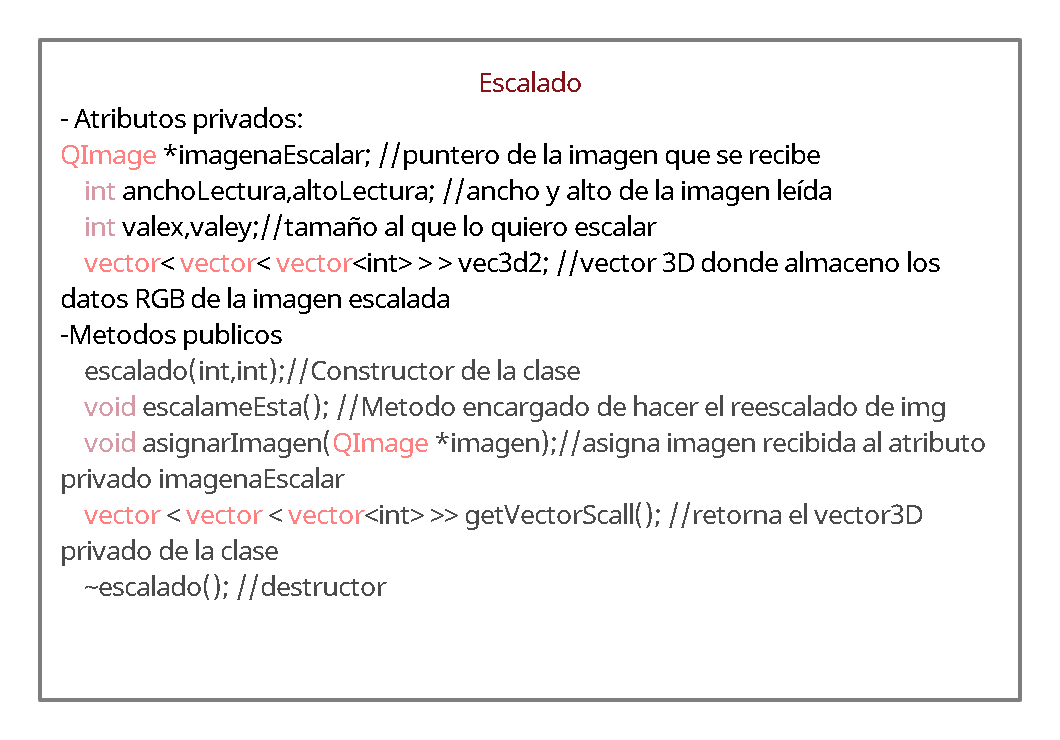
\includegraphics[width=8cm]{resources/esquemaEscalado.png}
\centering

\caption{esquema Clase escalado}
\end{figure}
\begin{figure}[h]
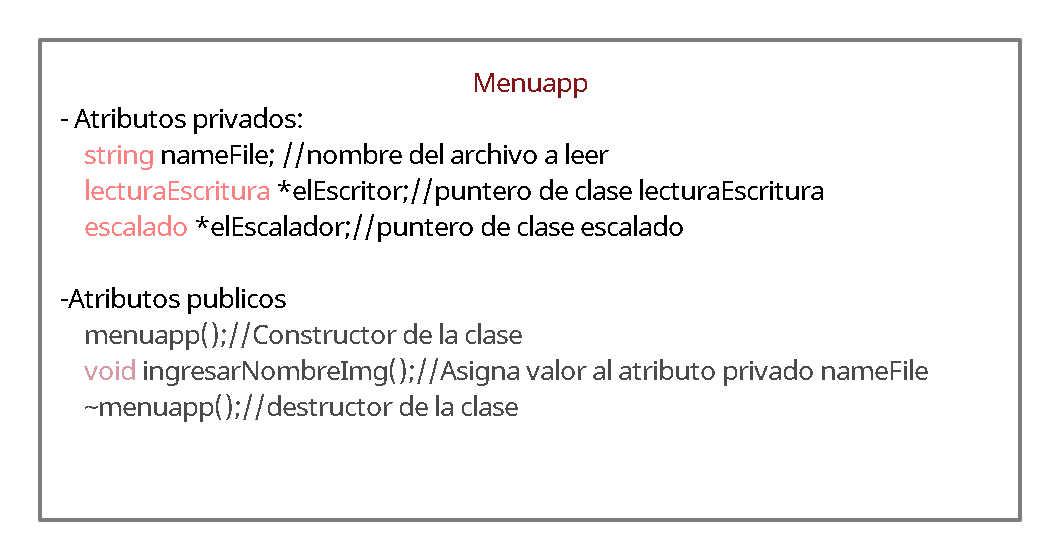
\includegraphics[width=8cm]{resources/esquemaMenuapp.png}
\centering

\caption{esquema Clase menuapp}
\end{figure}

\newpage
\section{Módulos de código de interacción}
\begin{lstlisting}[language=C++, caption=Intereacción de clases]
#include "menuapp.h"

menuapp::menuapp()
{
    ingresarNombreImg();
    elEscritor = new lecturaEscritura(nameFile.c_str());
    elEscalador = new escalado(elEscritor->getAncho(),elEscritor->getAlto());
    elEscalador->asignarImagen(elEscritor->getImagenFuente());
    elEscalador->escalameEsta();
    elEscritor->escribirTxt(elEscalador->getVectorScall());
}

void menuapp::ingresarNombreImg()
{
    cout << "------------------------------------------" << endl;
    cout << "+-+-+-+-+-+  BIENVENID@  +-+-+-+-+-+-+-+-+" << endl;
    cout << "Por favor ingrese el nombre de la imagen  " << endl;
    cout << "con su formato. Ejemplo: lolita.jpg" << endl;
    cout << "su respuesta:  ";
    cin >> nameFile;
}

menuapp::~menuapp()
{
    delete elEscritor;
    delete elEscalador;
}

\end{lstlisting}
\newpage
\section{Estructura del circuito}
\begin{figure}[h]
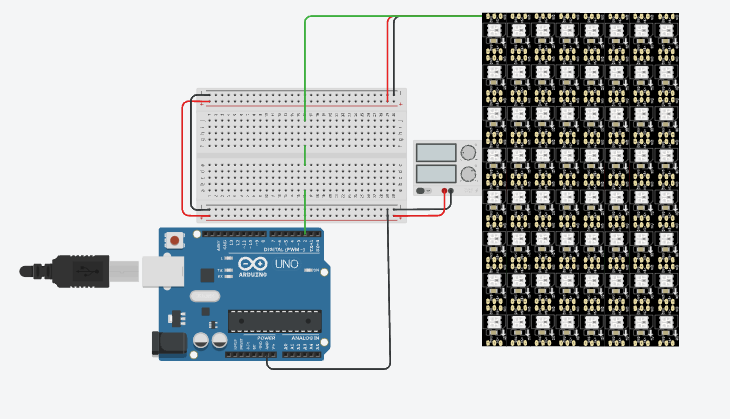
\includegraphics[width=12cm]{resources/circuito.PNG}
\centering
\caption{Circuito implementado}
\end{figure}
\newpage
\section{Problemas presentados durante la implementación}
Durante la implementación tuve varios inconvenientes. Las cosas tal y como las puse en el informe de análisis resultaron ser más complejas de lo que me esperaba. Primero que todo el escalar la imagen con ella ya guardada en un vector 3D (que era como lo tenia contemplado) resulto bastante engorroso y frustrante. Me perdía horrible para acceder a los datos de esa matriz 3d entonces opte por cambiar de metodología y transformar la imagen mientras la leo. El otro problema que tuve y el más frustrante de todos fue el de ampliar la imagen. En mi cabeza todo se veía muy lindo, la tenia clara pero no sabia como representar eso en el código, no sabia que condiciones tomar. Me estaba enredando horriblemente, tuve que dejar de programar ese día y al siguiente día fui capaz de plantear una solución
    

\end{document}